%%%%%%%%%%%%%%%%%%%%%%%%%%%%%%%%%%%%%%%%%%%%%%%%%%%%%%%%%%%%%%%%%%%%%%%%%%%%%%%%%%%%%%
% This LaTeX file was prepared by:
%       Rajat Subhra Chakraborty
%       Assistant Professor
%       Dept. of Computer Science and Engineering
%       IIT Kharagpur
%       Kharagpur, India - 721302
%       E-mail: rschakraborty@cse.iitkgp.ernet.in
%       Last Modified: 11th January, 2011
%%%%%%%%%%%%%%%%%%%%%%%%%%%%%%%%%%%%%%%%%%%%%%%%%%%%%%%%%%%%%%%%%%%%%%%%%%%%%%%%%%%%%%
\documentclass{article}
\usepackage[pdftex]{color,graphicx}
\usepackage{amsmath}
\usepackage{amssymb}
\usepackage{algorithm}
\usepackage{algorithmic}
\usepackage{enumerate}
\usepackage{syntonly}
\usepackage{multicol}
\usepackage{array}
%\usepackage[tight,footnotesize]{subfigure}
%\usepackage{stfloats}
%\usepackage{url}
%\usepackage{threeparttable}
%\usepackage{cite}
\usepackage{exam}

\paper{CS60004}  % <- do not include FC, FT etc
%\version{0}                     % <- for multiple choice exams
\subject{CS60004: Hardware Security}
\title{Mid-Term Examination}
\time{2}                      % <- number of hours: default is three
\semester{Spring}
\year{2015}                     % <- default is the current year
%\campus{Shanghai}
\fullmarks{40}
\note{Please answer all the questions. \newline
Special credit would be given for answers which are to-the-point.\\
 Please ensure that your handwriting is legible.\\
}

\begin{document}
\begin{center}
  \large{\bf Hardware Security\\[5mm]
    %MULTIPLE CHOICE QUESTIONS}\\[5mm]
    %Circle the preferred choice {\bf on the coloured answer sheet provided.
    }
\end{center}

\begin{questions}
\question Consider a field $GF(2^m)$ where $m$ is even. The field is constructed using an irreducible polynomial $P(x)=x^m+x^n+1$, where $n$ is odd, and $n < {m \over 2}$. Any element of the field can be expressed as $A(x)=\Sigma_{i=0}^{m-1}a_ix^i$, where the coefficients $a_i \in \{0,1\}$.  

\begin{enumerate}
\item We would like to perform the operation $C(x)=(A(x))^2 \mbox{mod }P(x)$. Derive the equations to express the $i^{th}$ coefficient of $C(x)$, denoted as $c_i$ where $0 \leq i \leq (m-1)$, in terms of the coefficients of $A(x)$. Split your derivation into the following four classes:
\begin{enumerate}
\item $i$ even, $i < n$ or $i \geq 2n$
\item $i$ even, $n < i < 2n$
\item $i$ odd, $i < n$
\item $i$ odd, $i \geq n$
\end{enumerate}

\item For a corresponding hardware realization for the above operation, what would be the type and number of gates required?
 
\item What would be the critical path (longest delay path) for the above hardware circuit? 
\end{enumerate}
\marks{10}

\question Professor Calculus wants to perform research in the field of designing efficient block ciphers like AES. In the process, he contemplates on developing new designs for the underlying S-Box for AES like ciphers. Suggest Prof Calculus appropriate feedbacks on the following design choices that he considers. Note that the underlying field structure is unaltered wrt. AES.
\begin{enumerate}
\item {\em Technique 1:} He considers to replace the AES S-Box by the function, $y=x^{1/2}$, where $x \in GF(2^4)^2$. 
\item {\em Technique 2:} He considers to replace the AES S-Box by the function, $y=x^{-2}$,  where $x \in GF(2^4)^2$.  
\item {\em Technique 3:} He considers performing the computation for the 
S-Box in two stages: 
$y_1=x^2$, $y=y_1^{-1}$,  where $x \in GF(2^4)^2$.  
\end{enumerate} 
Are each of the above techniques correct from the point of view of crytographic strength (ie, one should not follow a method which reduces classical security)?

For the techniques which you feel are justified help him to derive corresponding circuits. {\bf Assume that the inputs are already transformed to $GF(2^4)^2$. Also you need not decompose the fields further).} 
\marks{10}

\question Consider a toy cipher as shown in Fig.~\ref{sbox} implemented on a smart card. The cipher has a 4 bit plaintext which is not visible to the adversary. However, the adversary has access to the ciphertexts and also the corresponding power consumptions which are represented as integer values. The S-Box of the cipher is as in the following table: 

\begin{table}[h]
\begin{tabular}{ccccccccccccccccc}\hline
x &  0 & 1 & 2 & 3 & 4 & 5 & 6 & 7 & 8 & 9 & A & B & C & D & E & F\\
$S[X]$ & C & 5 & 6 & B & 9 & 0 & A & D & 3 & E & F & 8 & 4 & 7 & 1 & 2\\\hline
\end{tabular}\caption{The S-Box}
\end{table}

The adversary runs the encryptions several times until it obtains all the unique 16 ciphertext values (denoted as $C$) at least once. It also notes the corresponding power values denoted as $P$ which are denoted in the following table:

\begin{table}[h]
\begin{tabular}{ccccccccccccccccc}\hline
C & 0 & 1 & 2 & 3 & 4 & 5 & 6 & 7 & 8 & 9 & A & B & C & D & E & F\\
P & 10 & 15 & 20 & 5 & 10 & 5 & 5 & 15 & 15 & 5 & 10 & 10 & 0 & 15 & 10 & 10\\\hline
\end{tabular}\caption{The Power Profile}
\end{table}

\begin{enumerate}
\item You are told that the key is either $0101$ or $1010$. Apply the Difference-of-Mean (DOM) technique to determine which is the correct key byte. {\bf Target the MSB of the input of the S-Box.}
\item Define a hypothetical power vector by defining 
$h_P=HW(s)$, where $s$ is the value of the target register and $HW$ is the Hamming Weight. 
For both the above keys compute the hypothetical power vector for all the 
ciphertext values and compute the Pearson's Correlation between the hypothetical power and the actual power vector. Return the key with the highest correlation value. 

{\bf Remember that Pearson's correlation between two vectors $A$ and $B$, both of which have $n$ number of samples is computed as: 
$corr={{\Sigma_{i=1}^n(A[i]-\overline{A})(B[i]-\overline{B})}\over
{\Sigma_{i=1}^n(A[i]-\overline{A})^2\Sigma_{i=1}^n(B[i]-\overline{B})^2}}$. 
Here $\overline{A}$ and $\overline{B}$ are the means of the vectors $A$ and $B$.} 
\end{enumerate}
\marks{10}


\begin{figure}[h]
\centering
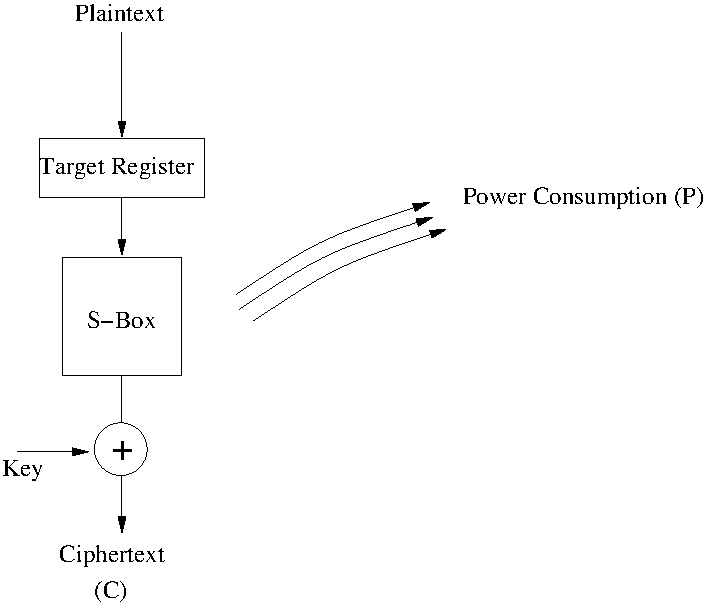
\includegraphics[width=2.5in]{figs/SBOXDPA}
%\epsfig{file= Images/isgreater.jpg, width=3.0in}
\caption{The Cipher under Attack}
\label{sbox}
\end{figure}

\question Consider an exponentiation algorithm $y = x^b$, where $b$ is a secret exponent which is of 8 bits. The exponents are denoted as $b_7, \ldots, b_0$. The exponent can be considered to be made of 2 nibbles (4-bits). An attacker is able to inject random faults in either of the two nibbles (when one nibble is affected the other is error free). Note that since the fault is random, some of the bits inside the faulty nibble may be unaffected too! The attacker obtains the results of $y = x^b$ and $y = x^{b^{\prime}}$, were $b^{\prime}$ is the faulty exponent under the above fault model. Develop an algorithm for the attacker to obtain the exponent bits. Also calculate the expected number of remaining exponents for one fault induction and two fault inductions.

{\bf Remember if $X$ is a random variable, expectation of $X$ is computed as $E(X)=\Sigma_i (x_ip_i)$, where $x_i$ is a possible value of the random variable $X$, and which occurs with probability $p_i$. The sample points are denoted by $i$.} 

\marks{10}

  


\end{questions}
\end{document}
